\documentclass{article}
\usepackage{biblatex}
\usepackage[margin=.5in]{geometry}
\usepackage{graphicx,wrapfig,lipsum}
\title{Arduino based Earthquake Detection System\quad\quad\quad\quad\quad\quad\quad\quad\quad\quad\quad\quad\quad\quad\quad\quad\quad\quad\quad (EDS) }
\author{Louise Carlo Salomon}
\date{March 2022}
\addbibresource{mybib.bib}

\begin{document}
\pagenumbering{gobble}
\maketitle
% \newpage
\textbf{\textit{Abstract-} Earthquake is the sudden release of strain energy in the earth's crust, resulting in waves of shaking that radiate outwards from the earthquake source.} 
\\\\





% hello \cite{einstein}
\section*{I. Introduction}
The Philippines, being situated in the Pacific Ring of Fire makes it vulnerable to frequent earthquakes and volcanic eruptions\cite*{ringOfFire}. It is evident what would happen to a big city when an unprecented massive earthquake were to happen, buildings collapsed, loss of life, loss of home, etc. This disaster can be mitigated by protection and accurate predication of earthquakes. But as of now, earthquake prediction techniques are still being developed and may still take a long time to use them practically. If, on the other hand, an earthquake warning system is made to alarm nearby residence that a massive earthquake is happening, then people can now act rationally to mitigate the earthquake hazard. \\

\noindent \underline{Earthquake} is the sudden release of strain energy in the earth's crust, resulting in waves of shaking that radiate outwards from the earthquake source. The rocks beneath the earth's crust crumbles when the friction between two blocks of the earth surprass their limit and thus allowing these blocks to slip past one another\cite*{earthquake}. The surface where they slip is called the fault or fault plane\cite*{SciEarth}. A fault, in geology is a planar or gently curved fracture in the rocks of Earth's crust, where compressional or tensional forces cause relative displacement of the rocks on the opposite sides of the fracture\cite*{fault}. The location where an earthquake starts is termed the focus or hypocentre and may be many kilometres deep within the earth. The point at the surface directly above the focus is called the earthquake epicentre\cite*{SciEarth}. When an earthquake occurs, intense vibrations, or seismic waves, spread out from the initial point of rupture (the focus) like ripples on a pond. These waves are what makes the ground shake and can travel large distances in all directions. Near the focus, the waves can be very large, making them extremely destructive endangering nearby civilization that could cost hundreds of lives\cite*{earthquake}.Sometimes an earthquake has foreshocks. These are smaller earthquakes that happen in the same place as the larger earthquake that follows. Researchers can't tell that an earthquake is a foreshock until the larger earthquake happens. The largest, main earthquake is called the mainshock. Mainshocks always have aftershocks that follow. Aftershocks are smaller earthquakes that occur afterwards in the same place as the mainshock. These aftershocks can occur for weeks, months and even for years depending on how big the mainshock is\cite*{SciEarth}.\\\\ 
\underline{Seismic Waves} are caused by the sudden movement of materials  within the Earth, such as slip along a fault during an earthquake.  Volcanic eruptions, explosions, landslides, avalanches, and even rushing riverscan also cause  seismic waves.     There 
\begin{wrapfigure}{r}{7cm}
    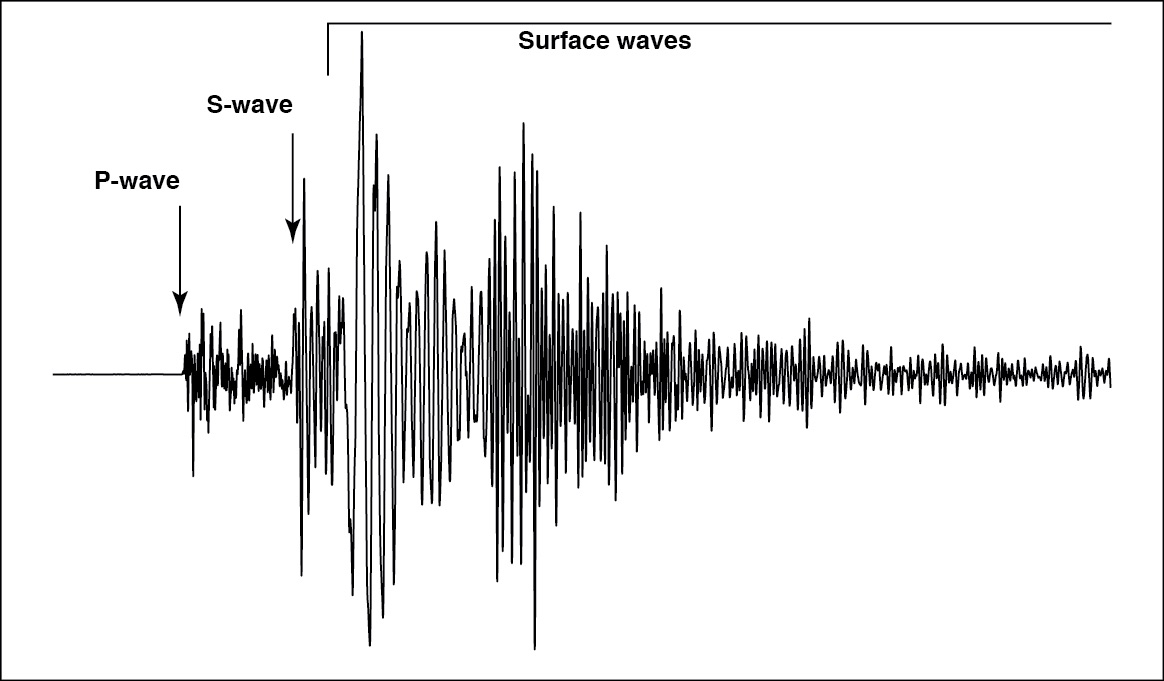
\includegraphics[width=7cm]{waves.jpg}
    \caption{The body waves (P and S) and surface waves recorded by a seismometer.}\label{wrap-fig:1}
\end{wrapfigure} 
 are several different kinds of seismic waves, and they all move in different ways.  The two main types of waves are body waves and surface waves. Body waves can travel through the Earth's inner layers, but surface waves can only move along the surface of the planet like ripples on water. Earthquakes send out seismic energy as both body and surface waves. These seismic waves can be precisisely recoreded using seismometer inside a seismograph\cite*{SiesWav}. \textit{see figure 1.} \\

\noindent Large organizations use complex systems to detect earthquakes and measure the magnitude of the earthquake was. But also, there are small and less complex chips that can be used to detect and measure the magnitude of an earthquake. Here accelerometer MPU6050 6-axis module is used to detect ground vibration with high persision. The MPU6050 accelerometer uses the Micro Electro Mechanical Technology to determine the acceleration of the three x, y, and z axis. Returning 16-bit adc of raw data to the microcontroller to process and convert to useful data for the program to use.



\newpage

\printbibliography
\end{document}
